\documentclass[12pt]{cover_letter}

\usepackage{pdfpages}

\begin{document}
  \begin{letter}{Apple}

    \opening{Dear Apple hiring manager,}

    % Sets the current page style to fancy (must happen after "opening")
    \thispagestyle{fancy}

    Your \textit{Technology Investigation Product Design Internship} posting found on the Georgia Tech CareerBuzz website interests me. A background on extra-curricular competition teams has given me extensive experience in 3D CAD, design for manufacture, and rapid prototyping, which would allow me to make meaningful contributions on your product design team.

    I taught myself to use CAD as a seventh grader on a high school FIRST robotics team. While the team had never used CAD before, I envisioned a role for myself to help design, manufacture, and iterate more efficiently and precisely using 3D CAD. Working with professional machine shops honed my ability to create unambiguous engineering drawings while the short, six-week build period taught me efficient design. In particular, I improved my ability to rapidly ideate and design for ease of manufacture. I became particularly adept in using Dassault Solidworks and both designing for and manufacturing with our in-house manual mill, manual lathe, and Haas CNC router. By my final year, at night I would design a prototype to solve a problem or test an idea, begin manufacturing on our CNC router at the next team meeting, and have a functioning concept by the meeting's conclusion.

    My work at Georgia Tech has cemented my desire to work in a design and development role. I thrived in "ME2110: Creative Designs and Design", a design competition class where my team created three complete iterations of our mechanism that placed 7th out of 60. By focusing our efforts on a CAD model that exploited laser-cut plywood, we were able to adjust and upgrade quickly and easily. I genuinely love design, iteration, design for manufacture.

    Attached you will find my resume; it contains further descriptions of my work on Georgia Tech's FSAE and robotics teams and my high school robotics team. I would be happy to answer further questions by email at \href{mailto:michael.bick@gatech.edu}{\nolinkurl{michael.bick@gatech.edu}}.

    \closing{Sincerely,}

  \end{letter}

  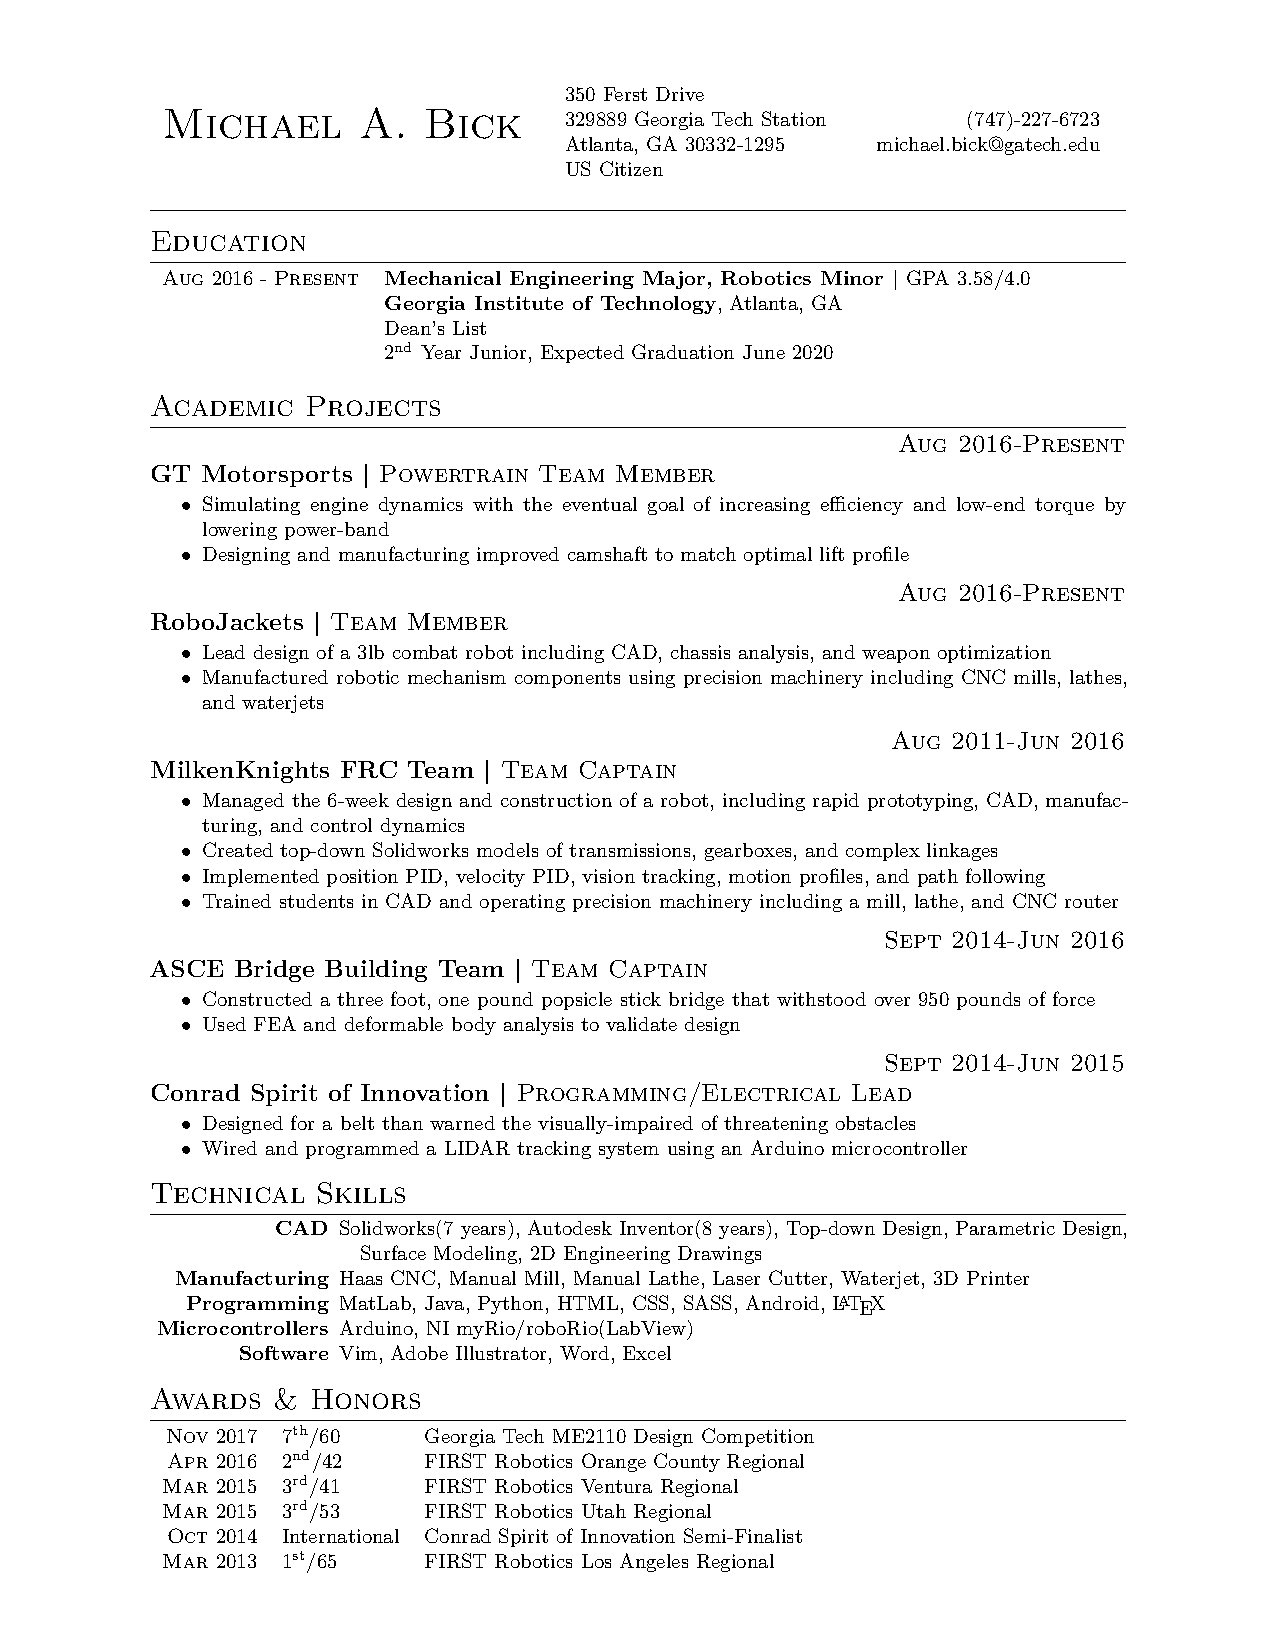
\includepdf[pages=-]{../../resumes/resume.pdf}
\end{document}
